\section{RefreshMgr Class Reference}
\label{classRefreshMgr}\index{RefreshMgr@{RefreshMgr}}
{\tt \#include $<$refresh\_\-manager.h$>$}

Inheritance diagram for RefreshMgr:\nopagebreak
\begin{figure}[H]
\begin{center}
\leavevmode
\includegraphics[width=146pt]{classRefreshMgr__inherit__graph}
\end{center}
\end{figure}
Collaboration diagram for RefreshMgr:\nopagebreak
\begin{figure}[H]
\begin{center}
\leavevmode
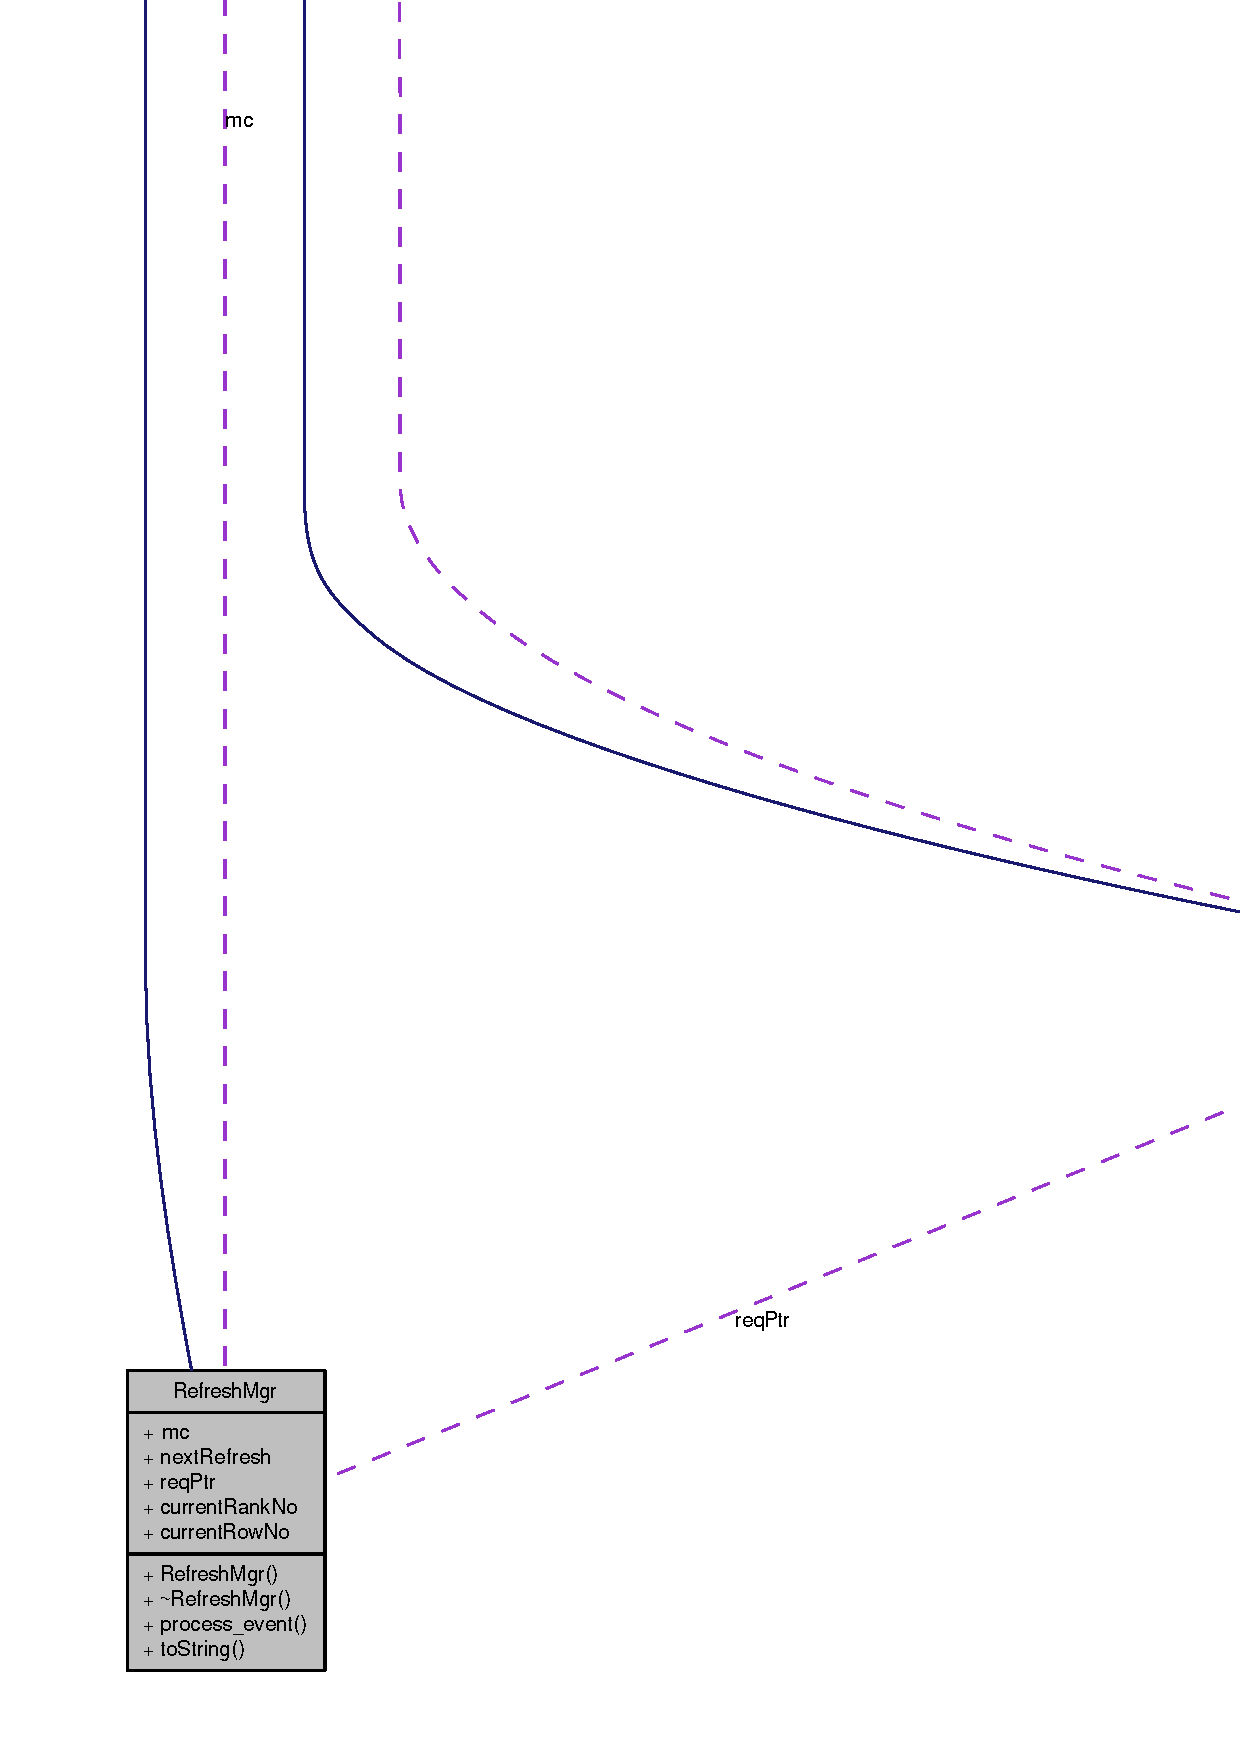
\includegraphics[width=400pt]{classRefreshMgr__coll__graph}
\end{center}
\end{figure}
\subsection*{Public Member Functions}
\begin{CompactItemize}
\item 
{\bf RefreshMgr} ()
\item 
{\bf $\sim$RefreshMgr} ()
\item 
void {\bf process\_\-event} ({\bf IrisEvent} $\ast$e)
\item 
std::string {\bf toString} ()
\end{CompactItemize}
\subsection*{Public Attributes}
\begin{CompactItemize}
\item 
{\bf Component} $\ast$ {\bf mc}
\item 
{\bf Time} {\bf nextRefresh}
\item 
{\bf RequestHandler} $\ast$ {\bf reqPtr}
\item 
unsigned int {\bf currentRankNo}
\item 
unsigned int {\bf currentRowNo}
\end{CompactItemize}


\subsection{Detailed Description}


Definition at line 44 of file refresh\_\-manager.h.

\subsection{Constructor \& Destructor Documentation}
\index{RefreshMgr@{RefreshMgr}!RefreshMgr@{RefreshMgr}}
\index{RefreshMgr@{RefreshMgr}!RefreshMgr@{RefreshMgr}}
\subsubsection[{RefreshMgr}]{\setlength{\rightskip}{0pt plus 5cm}RefreshMgr::RefreshMgr ()}\label{classRefreshMgr_5a2c872aa68b6cb67db561a030893ef9}




Definition at line 39 of file refresh\_\-manager.cc.

References currentRankNo, currentRowNo, and nextRefresh.\index{RefreshMgr@{RefreshMgr}!$\sim$RefreshMgr@{$\sim$RefreshMgr}}
\index{$\sim$RefreshMgr@{$\sim$RefreshMgr}!RefreshMgr@{RefreshMgr}}
\subsubsection[{$\sim$RefreshMgr}]{\setlength{\rightskip}{0pt plus 5cm}RefreshMgr::$\sim$RefreshMgr ()}\label{classRefreshMgr_52a8a561efe0357f2961f9a148919136}




Definition at line 53 of file refresh\_\-manager.cc.

\subsection{Member Function Documentation}
\index{RefreshMgr@{RefreshMgr}!process\_\-event@{process\_\-event}}
\index{process\_\-event@{process\_\-event}!RefreshMgr@{RefreshMgr}}
\subsubsection[{process\_\-event}]{\setlength{\rightskip}{0pt plus 5cm}void RefreshMgr::process\_\-event ({\bf IrisEvent} $\ast$ {\em e})}\label{classRefreshMgr_19d89c100f78a655bd7860111755128c}




Definition at line 65 of file refresh\_\-manager.cc.

References RequestHandler::busHandler, BusHandler::cmdIssuer, Request::cmdType, currentRankNo, currentRowNo, IrisEvent::dst, BusHandler::LowLevelCmdGen(), nextRefresh, NO\_\-OF\_\-CHANNELS, NO\_\-OF\_\-RANKS, NO\_\-OF\_\-ROWS, Simulator::Now(), CmdIssuer::process\_\-event(), Request::rankNo, REFRESH, REFRESH\_\-INC, reqPtr, ROW\_\-SIZE, Request::rowNo, Simulator::Schedule(), IrisEvent::src, and START.

Referenced by MC::StartRefresh().

Here is the caller graph for this function:\nopagebreak
\begin{figure}[H]
\begin{center}
\leavevmode
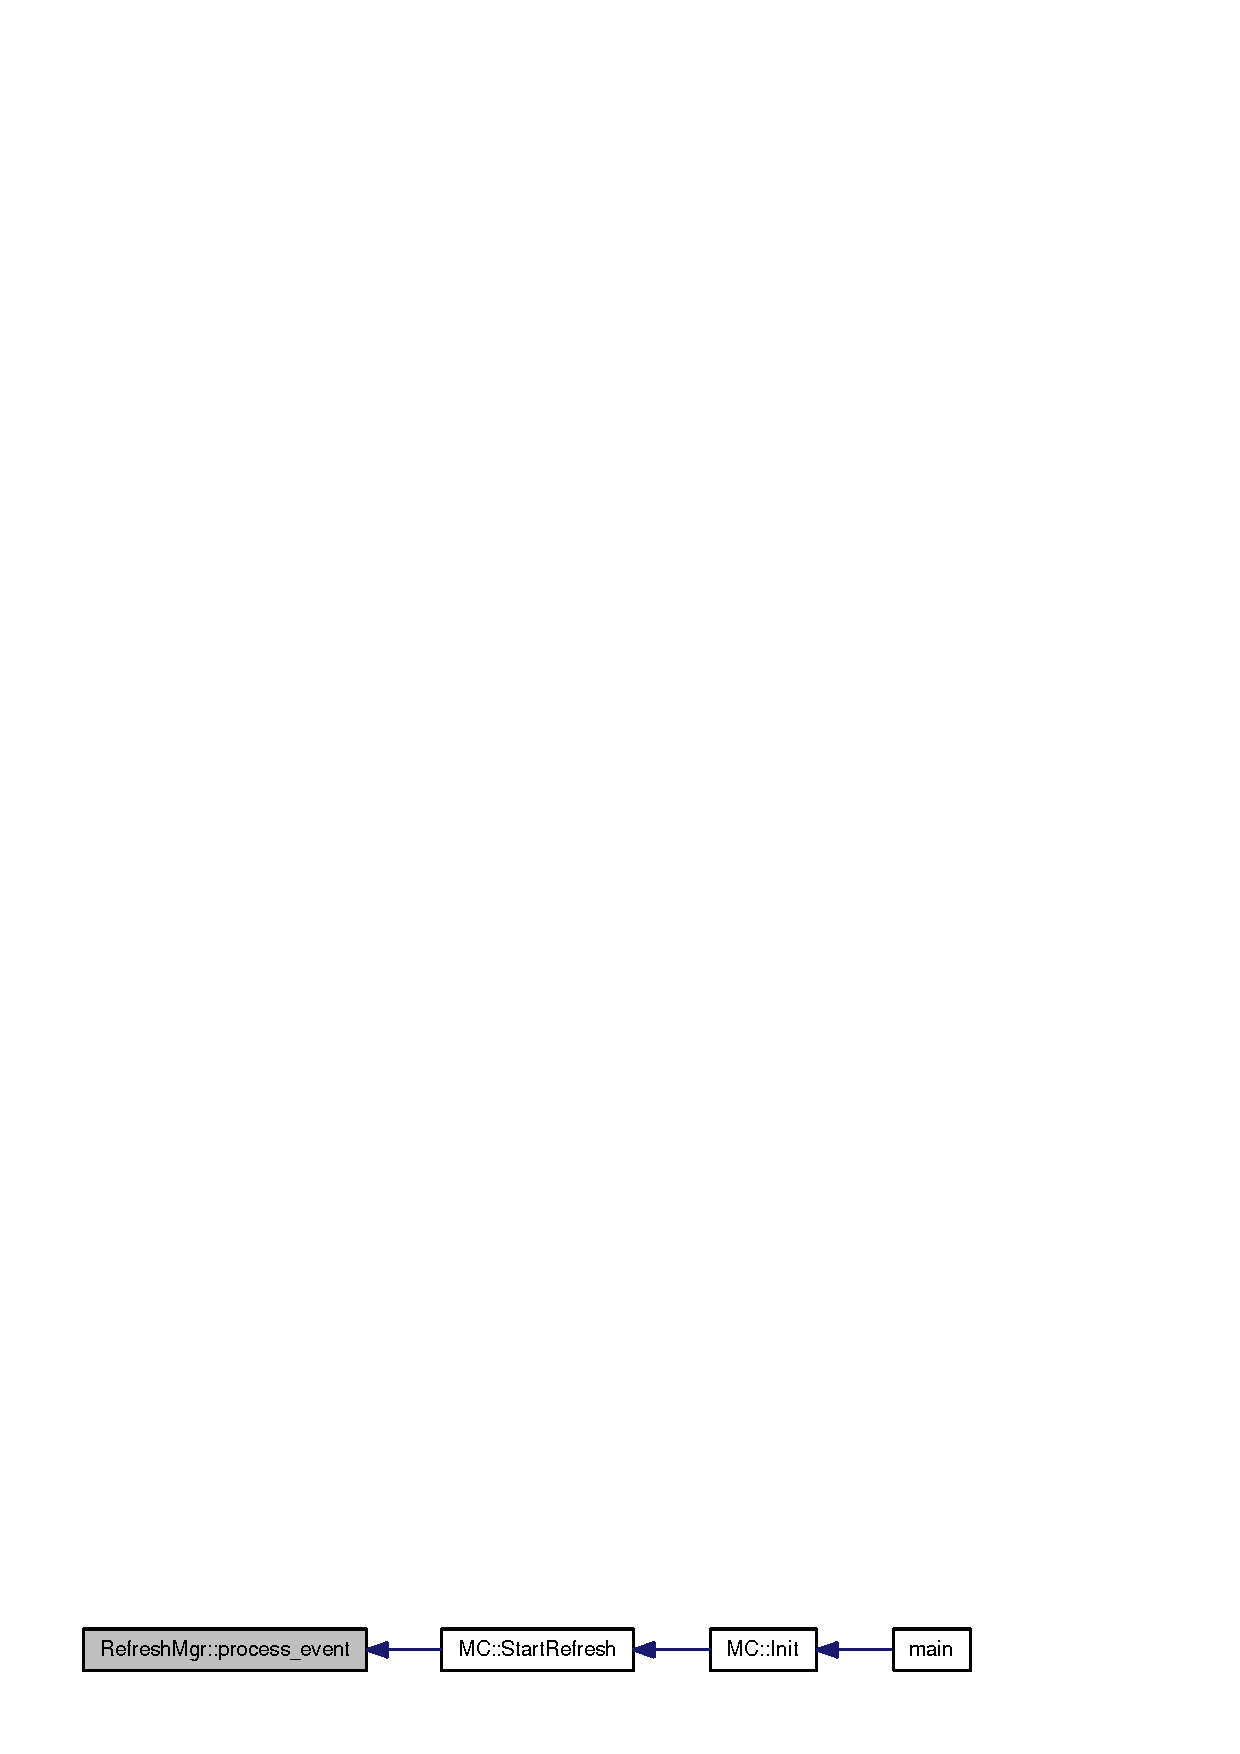
\includegraphics[width=235pt]{classRefreshMgr_19d89c100f78a655bd7860111755128c_icgraph}
\end{center}
\end{figure}
\index{RefreshMgr@{RefreshMgr}!toString@{toString}}
\index{toString@{toString}!RefreshMgr@{RefreshMgr}}
\subsubsection[{toString}]{\setlength{\rightskip}{0pt plus 5cm}std::string RefreshMgr::toString ()}\label{classRefreshMgr_73f53993e11a1bac1d4c7203a61b6b81}




\subsection{Member Data Documentation}
\index{RefreshMgr@{RefreshMgr}!currentRankNo@{currentRankNo}}
\index{currentRankNo@{currentRankNo}!RefreshMgr@{RefreshMgr}}
\subsubsection[{currentRankNo}]{\setlength{\rightskip}{0pt plus 5cm}unsigned int {\bf RefreshMgr::currentRankNo}}\label{classRefreshMgr_bd56a4843e3bf40bc87192a74f51b337}




Definition at line 53 of file refresh\_\-manager.h.

Referenced by process\_\-event(), and RefreshMgr().\index{RefreshMgr@{RefreshMgr}!currentRowNo@{currentRowNo}}
\index{currentRowNo@{currentRowNo}!RefreshMgr@{RefreshMgr}}
\subsubsection[{currentRowNo}]{\setlength{\rightskip}{0pt plus 5cm}unsigned int {\bf RefreshMgr::currentRowNo}}\label{classRefreshMgr_d52556a29b0438070616d85fed03a58f}




Definition at line 54 of file refresh\_\-manager.h.

Referenced by process\_\-event(), and RefreshMgr().\index{RefreshMgr@{RefreshMgr}!mc@{mc}}
\index{mc@{mc}!RefreshMgr@{RefreshMgr}}
\subsubsection[{mc}]{\setlength{\rightskip}{0pt plus 5cm}{\bf Component}$\ast$ {\bf RefreshMgr::mc}}\label{classRefreshMgr_5ef603ac3e0216fa892f74bef4c736a3}




Definition at line 49 of file refresh\_\-manager.h.

Referenced by MC::Init().\index{RefreshMgr@{RefreshMgr}!nextRefresh@{nextRefresh}}
\index{nextRefresh@{nextRefresh}!RefreshMgr@{RefreshMgr}}
\subsubsection[{nextRefresh}]{\setlength{\rightskip}{0pt plus 5cm}{\bf Time} {\bf RefreshMgr::nextRefresh}}\label{classRefreshMgr_ea259f790c8c353f3c61c3d56a5ecc9a}




Definition at line 50 of file refresh\_\-manager.h.

Referenced by process\_\-event(), RefreshMgr(), and MC::StartRefresh().\index{RefreshMgr@{RefreshMgr}!reqPtr@{reqPtr}}
\index{reqPtr@{reqPtr}!RefreshMgr@{RefreshMgr}}
\subsubsection[{reqPtr}]{\setlength{\rightskip}{0pt plus 5cm}{\bf RequestHandler}$\ast$ {\bf RefreshMgr::reqPtr}}\label{classRefreshMgr_59369708c3b99c76377847da760d635f}




Definition at line 51 of file refresh\_\-manager.h.

Referenced by MC::Init(), and process\_\-event().

The documentation for this class was generated from the following files:\begin{CompactItemize}
\item 
{\bf refresh\_\-manager.h}\item 
{\bf refresh\_\-manager.cc}\end{CompactItemize}
